\documentclass{article}\usepackage[]{graphicx}\usepackage[]{color}
%% maxwidth is the original width if it is less than linewidth
%% otherwise use linewidth (to make sure the graphics do not exceed the margin)
\makeatletter
\def\maxwidth{ %
  \ifdim\Gin@nat@width>\linewidth
    \linewidth
  \else
    \Gin@nat@width
  \fi
}
\makeatother

\definecolor{fgcolor}{rgb}{0.345, 0.345, 0.345}
\newcommand{\hlnum}[1]{\textcolor[rgb]{0.686,0.059,0.569}{#1}}%
\newcommand{\hlstr}[1]{\textcolor[rgb]{0.192,0.494,0.8}{#1}}%
\newcommand{\hlcom}[1]{\textcolor[rgb]{0.678,0.584,0.686}{\textit{#1}}}%
\newcommand{\hlopt}[1]{\textcolor[rgb]{0,0,0}{#1}}%
\newcommand{\hlstd}[1]{\textcolor[rgb]{0.345,0.345,0.345}{#1}}%
\newcommand{\hlkwa}[1]{\textcolor[rgb]{0.161,0.373,0.58}{\textbf{#1}}}%
\newcommand{\hlkwb}[1]{\textcolor[rgb]{0.69,0.353,0.396}{#1}}%
\newcommand{\hlkwc}[1]{\textcolor[rgb]{0.333,0.667,0.333}{#1}}%
\newcommand{\hlkwd}[1]{\textcolor[rgb]{0.737,0.353,0.396}{\textbf{#1}}}%
\let\hlipl\hlkwb

\usepackage{framed}
\makeatletter
\newenvironment{kframe}{%
 \def\at@end@of@kframe{}%
 \ifinner\ifhmode%
  \def\at@end@of@kframe{\end{minipage}}%
  \begin{minipage}{\columnwidth}%
 \fi\fi%
 \def\FrameCommand##1{\hskip\@totalleftmargin \hskip-\fboxsep
 \colorbox{shadecolor}{##1}\hskip-\fboxsep
     % There is no \\@totalrightmargin, so:
     \hskip-\linewidth \hskip-\@totalleftmargin \hskip\columnwidth}%
 \MakeFramed {\advance\hsize-\width
   \@totalleftmargin\z@ \linewidth\hsize
   \@setminipage}}%
 {\par\unskip\endMakeFramed%
 \at@end@of@kframe}
\makeatother

\definecolor{shadecolor}{rgb}{.97, .97, .97}
\definecolor{messagecolor}{rgb}{0, 0, 0}
\definecolor{warningcolor}{rgb}{1, 0, 1}
\definecolor{errorcolor}{rgb}{1, 0, 0}
\newenvironment{knitrout}{}{} % an empty environment to be redefined in TeX

\usepackage{alltt}
\usepackage{gensymb}
\usepackage{hyperref}

\title{Visual Presentation of Data using R}



\IfFileExists{upquote.sty}{\usepackage{upquote}}{}
\begin{document}
\maketitle

\section{The Perfect Graphic}

\subsection{Best Practices}

There is no such thing as the perfect graphic, but there are conventions that can be used to guide us to create accurtate, accessible, and visually pleasing grahics. But like many things, it takes some practices. 

Here are some general rules:

\begin{itemize}
  \item Be sure that you introduce the graphic/table with text -- i.e. text first, then graphic. 
  \item Cite the graphic/table with a figure or table number. 
  \item Describe the graphic/table with a caption.
  \item Manage data range and transformations to effectively analyze and display the data.
  \item Make sure the axes are labeled with appropriate units
  \item Manage axis labels, value font size, and orientation to make them easy to reads.
  \item Avoid graphic titles unless you have more than one panel, i.e. graphics that are side by side or on top of each other. 
  \item Do not connect data points with lines unless you can 'reasonable' interpolate between the points, e.g. a continous data set with some level of autocorrelation. 
  \item Are the graphics accessible?  For example, black and white can be better than color in terms of accessibility (universal design) and sustainability. 
  \item Use the caption to describe what the reader is supposed to see in the figure. 
\end{itemize}

\subsection{How to Cite Software}

In the text, students often make a bigger deal out the software than it deserses. Probably, because we feel like we climbed a big mountain to have some success and want demonstrate that. However, in general, environmental scientists downplay the software, unless they wrote a specific function or library. 

Thus, for our purposes, the following is usually sufficient...

\noindent ``Statistical analysis was conducted using using R (CRAN 2019)."

You don't need to mention how you imported it, used Rstudio, or talk about the functions. In the text, you might mention that you used a linear model, regression, analysis of variance (AOV), but the details of the R code is usually not mentioned.

However, you should also cite the program in your endnote: 

\smallskip
To cite R in publications use:

\medskip
\noindent R Core Team. 2017. R: A language and environment for statistical computing. R Foundation for Statistical Computing, Vienna, Austria. URL \url{https://www.R-project.org/}.

\smallskip

\noindent You can get an updated version of the citation using the following function in R: citation(). Although the format isn't quite the same.
  

\subsection{Reporting Results}

In statistics, we reject the null hypothesis -- and don't prove anything. So, we need to be careful how we report our results. 

First, when we report statistics, do not report the p-value if the result in non-significant. Just report that null hypothesis cannot be rejected. If the p-value is less then 0.001, just report it as `p $<$ 0.001'. If the p-value is between 0.05 and 0.001, then I suggest you report the actual value (rounded to the nearest one-hundredth or thousandth as appropriate. 

Second, when we report the r$^2$ value, round to the nearest one-hundredth and describe it as the 'amount of variation explained by the model'. In fact, if you multiply by 100, it's can thought of as a percent variation explained.

Finally, avoid making the statistics the subject of the sentence! Describe the results as the subject/verb and then add a parenthetical about the stats, e.g.

\noindent Water quality declined through the study period (p = 0.03; r$^2$ = 0.09), although little of the variation was explained by the model. 

\section{Exploring the Histogram}

Data exploration can include many steps, but starting with a histogram gives the researcher the ability to evaluate the distribution of the data.

Below is a default histogram for TMAX values, where we might be able to visually how normally distributed the data might be.

\begin{knitrout}
\definecolor{shadecolor}{rgb}{0.969, 0.969, 0.969}\color{fgcolor}\begin{kframe}
\begin{alltt}
\hlkwd{hist}\hlstd{(MonthlyTMAXMean}\hlopt{$}\hlstd{TMAX)}
\end{alltt}
\end{kframe}
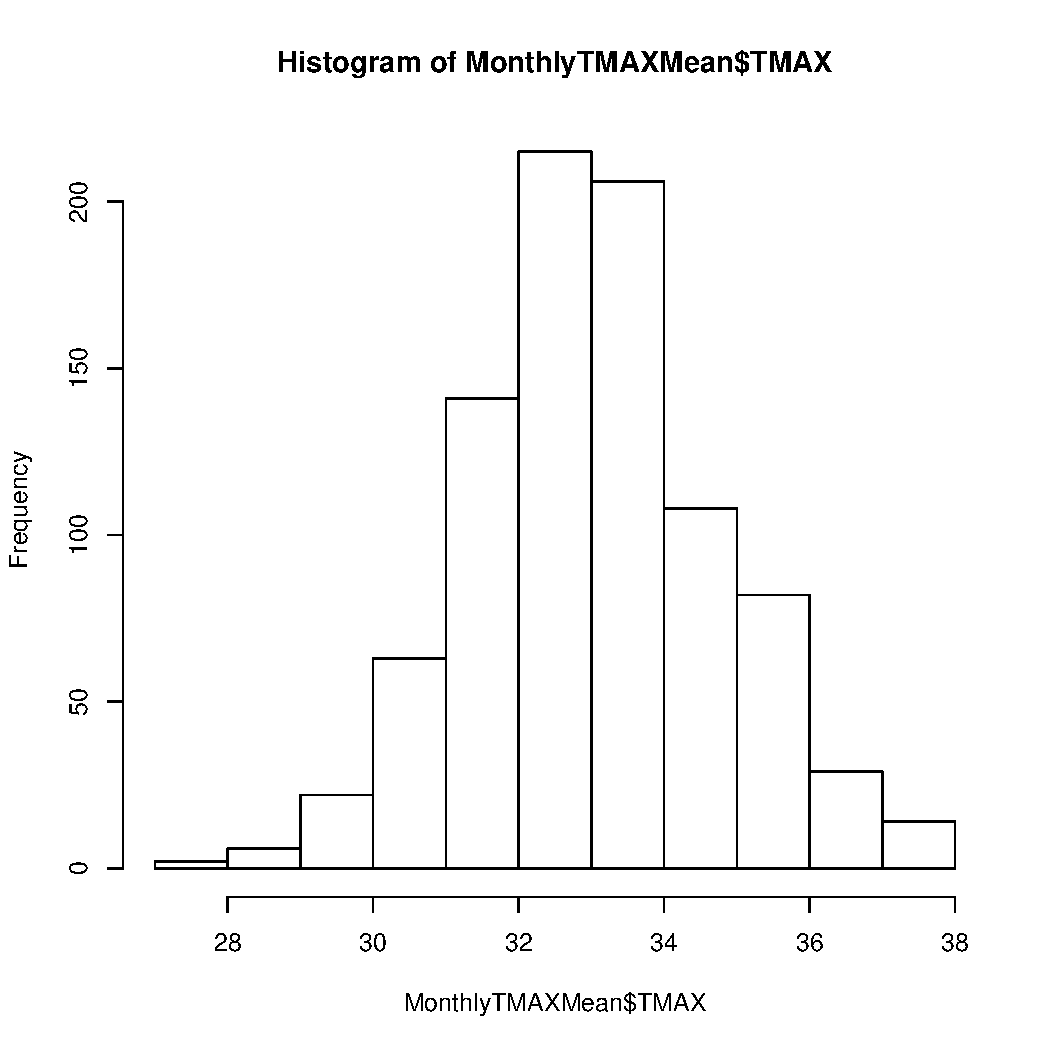
\includegraphics[width=\maxwidth]{figure/unnamed-chunk-2-1} 

\end{knitrout}

The default graphic is hideous -- so, let's start fixing it. 

\subsection{Title and Axis Labels}

For stand alone figures, we usually add titles, but in papers and lab reports it's a good practice to remove the title and use the caption to describe the graphic. Changes to the title can be made with arguments within the plot command, i.e. `main=NULL'.

In addition, we can change the x-axis label, with the 'xlab' argument. Specifying the units is also required. And in this case, we want to add the \degree symbol and create a text string with the axis label in quotes that can be referenced in the hist() funtion. 

\begin{knitrout}
\definecolor{shadecolor}{rgb}{0.969, 0.969, 0.969}\color{fgcolor}\begin{kframe}
\begin{alltt}
\hlstd{TMAXlabel} \hlkwb{<-} \hlstr{"Maximum Temperature (°C)"}
\hlkwd{hist}\hlstd{(MonthlyTMAXMean}\hlopt{$}\hlstd{TMAX,} \hlkwc{main}\hlstd{=}\hlkwa{NULL}\hlstd{,} \hlkwc{xlab}\hlstd{=TMAXlabel)}
\end{alltt}
\end{kframe}\begin{figure}
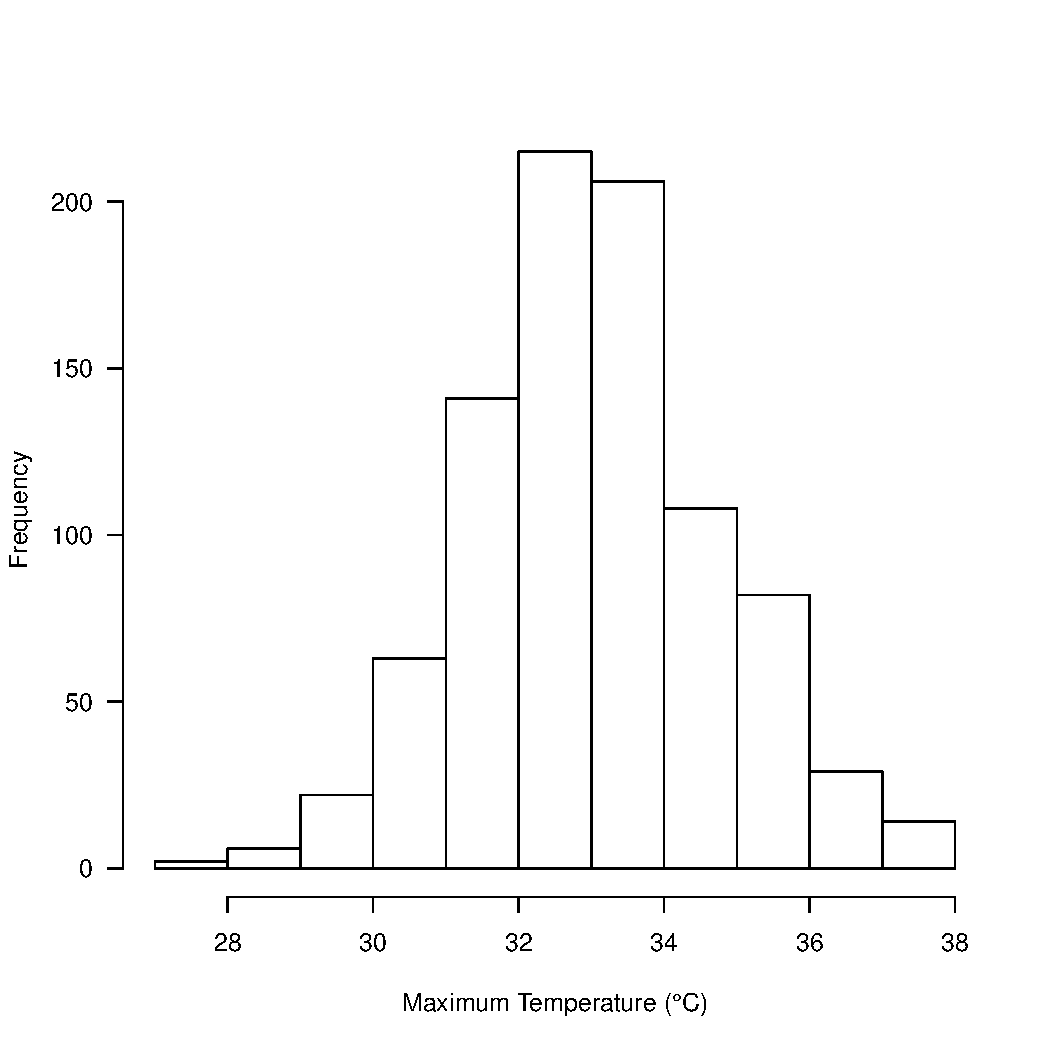
\includegraphics[width=\maxwidth]{figure/unnamed-chunk-3-1} \caption[Histogram of Maximum Temperatures (°C) (XXX, Thailand, 1940-2018)]{Histogram of Maximum Temperatures (°C) (XXX, Thailand, 1940-2018)}\label{fig:unnamed-chunk-3}
\end{figure}


\end{knitrout}
\clearpage
\subsection{Putting Multiple Figures in a Row}

To create two graphics in one row, we can change the graphic parameters with the par() function. In this case, we'll create two column panels in one row using the 'mfrow' option and a vector that defines the number of rows and the number of columns. It's often a good idea to set the graphic parameter back to the default afterwards. In this case, I added a title because we have a panel with two graphics. Often people will put letters, e.g. A and B to refer to each one separately, but I prefer to put the actually description in the title, so the reader doesn't have to go back and forth between the caption and the figures.

\begin{knitrout}
\definecolor{shadecolor}{rgb}{0.969, 0.969, 0.969}\color{fgcolor}\begin{kframe}
\begin{alltt}
\hlkwd{par}\hlstd{(}\hlkwc{mfrow}\hlstd{=}\hlkwd{c}\hlstd{(}\hlnum{1}\hlstd{,}\hlnum{2}\hlstd{))}
\hlkwd{hist}\hlstd{(MonthlyTMAXMean}\hlopt{$}\hlstd{TMAX,} \hlkwc{main}\hlstd{=}\hlstr{'Maximum Temperature'}\hlstd{,} \hlkwc{xlab}\hlstd{=TMAXlabel)}
\hlstd{TMINlabel} \hlkwb{<-} \hlstr{"Minimum Temperature (°C)"}
\hlkwd{hist}\hlstd{(MonthlyTMINMean}\hlopt{$}\hlstd{TMIN,} \hlkwc{main}\hlstd{=}\hlstr{'Minimum Temperature'}\hlstd{,} \hlkwc{xlab}\hlstd{=TMINlabel)}
\end{alltt}
\end{kframe}\begin{figure}
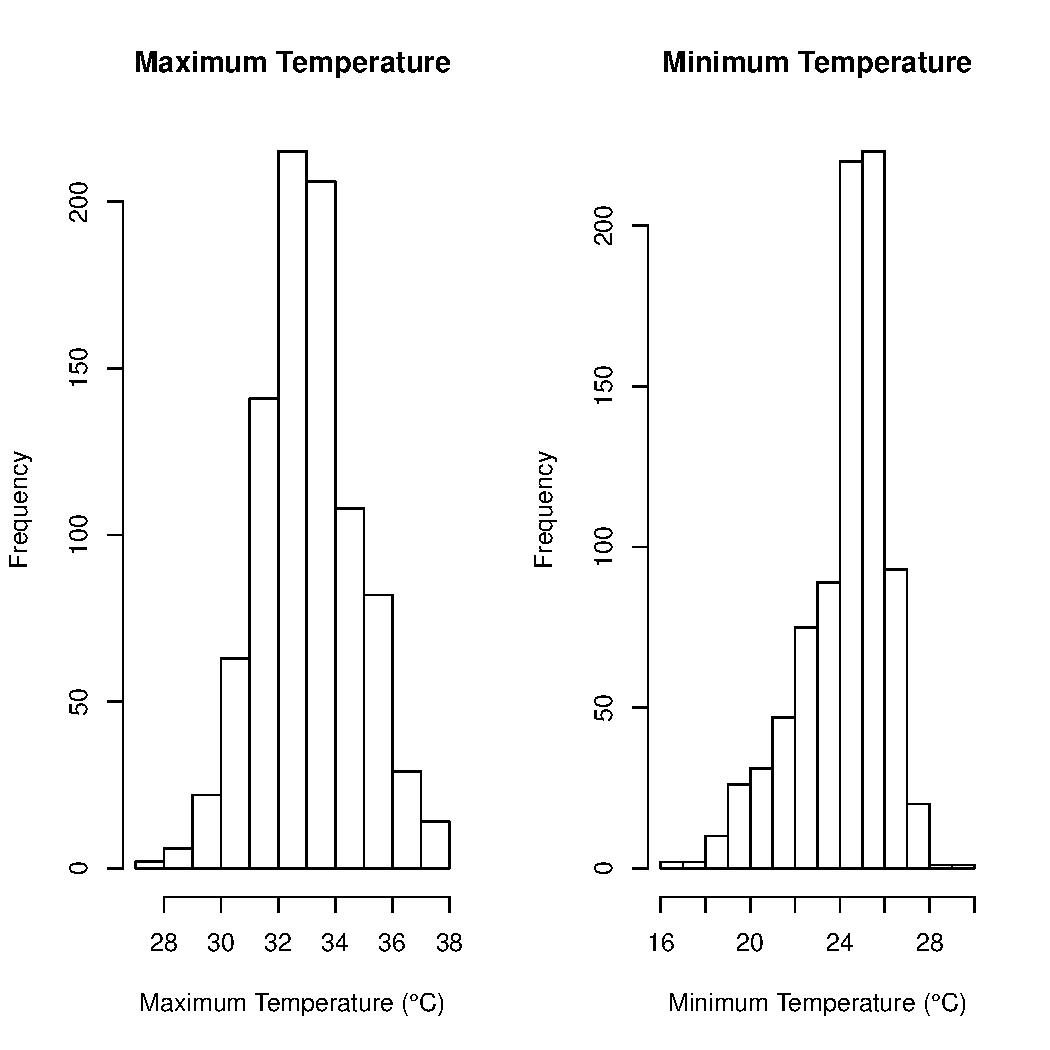
\includegraphics[width=\maxwidth]{figure/unnamed-chunk-4-1} \caption[Mean monthly maximum and minimum tempetures (C) ((XXX, Thailand, 1940-2018))]{Mean monthly maximum and minimum tempetures (C) ((XXX, Thailand, 1940-2018))}\label{fig:unnamed-chunk-4}
\end{figure}

\begin{kframe}\begin{alltt}
\hlkwd{par}\hlstd{(}\hlkwc{mfrow}\hlstd{=}\hlkwd{c}\hlstd{(}\hlnum{1}\hlstd{,}\hlnum{1}\hlstd{))}
\end{alltt}
\end{kframe}
\end{knitrout}
\newpage
Because the figure is rather distorted, I have constrained the size using a fig.height and fig.width option. 

\begin{knitrout}
\definecolor{shadecolor}{rgb}{0.969, 0.969, 0.969}\color{fgcolor}\begin{kframe}
\begin{alltt}
\hlkwd{par}\hlstd{(}\hlkwc{mfrow}\hlstd{=}\hlkwd{c}\hlstd{(}\hlnum{1}\hlstd{,}\hlnum{2}\hlstd{))}
\hlkwd{hist}\hlstd{(MonthlyTMAXMean}\hlopt{$}\hlstd{TMAX,} \hlkwc{main}\hlstd{=}\hlstr{'Monthly Maximum Temperature'}\hlstd{,} \hlkwc{xlab}\hlstd{=TMAXlabel)}
\hlstd{TMINlabel} \hlkwb{<-} \hlstr{"Minimum Temperature (°C)"}
\hlkwd{hist}\hlstd{(MonthlyTMINMean}\hlopt{$}\hlstd{TMIN,} \hlkwc{main}\hlstd{=}\hlstr{'Monthly Minimum Temperature'}\hlstd{,} \hlkwc{xlab}\hlstd{=TMINlabel)}
\end{alltt}
\end{kframe}\begin{figure}
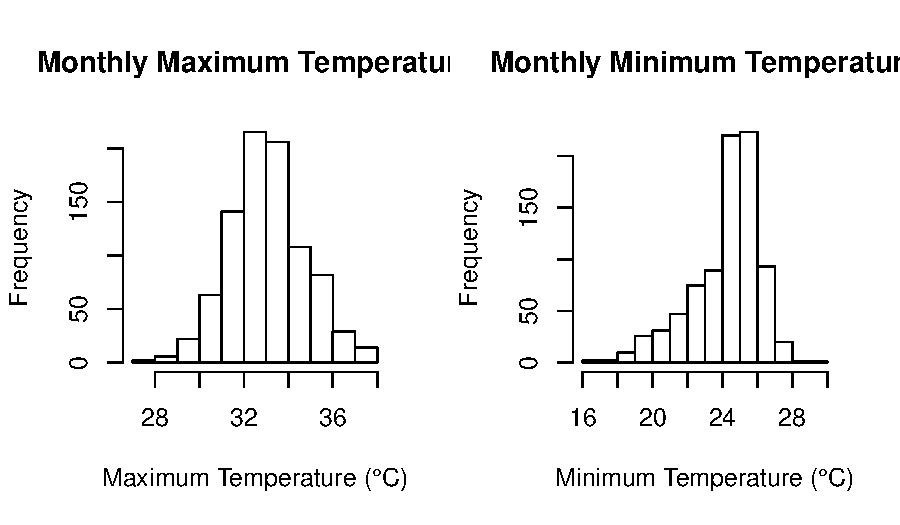
\includegraphics[width=\maxwidth]{figure/unnamed-chunk-5-1} \caption[Mean monthly maximum and minimum tempetures (C) ((XXX, Thailand, 1940-2018))]{Mean monthly maximum and minimum tempetures (C) ((XXX, Thailand, 1940-2018))}\label{fig:unnamed-chunk-5}
\end{figure}

\begin{kframe}\begin{alltt}
\hlkwd{par}\hlstd{(}\hlkwc{mfrow}\hlstd{=}\hlkwd{c}\hlstd{(}\hlnum{1}\hlstd{,}\hlnum{1}\hlstd{))}
\end{alltt}
\end{kframe}
\end{knitrout}

\section{Boxplot}

Box plots are great ways to display quantitative data from controlled experiments. For example, if you had high and low treatment categories and measured some response. Let's use the following example, ants colonies collected from three locations farm, grassland, and forest. 

\begin{knitrout}
\definecolor{shadecolor}{rgb}{0.969, 0.969, 0.969}\color{fgcolor}\begin{figure}
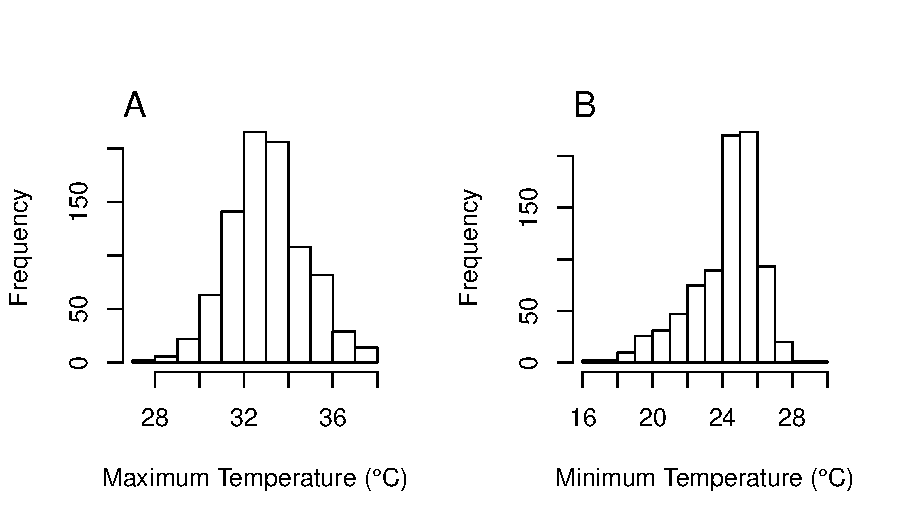
\includegraphics[width=\maxwidth]{figure/unnamed-chunk-6-1} \caption[Number of ant colonies by habitat type]{Number of ant colonies by habitat type}\label{fig:unnamed-chunk-6}
\end{figure}


\end{knitrout}
\newpage
\section{Scatter Plot -- Non-time series}

%For scatter plots, which are more common, we use the same principles:


\subsection{Scatter Plot -- Time Series}

Time series data sets often require special treatment. For example, data are often autocorrelated, thus data can be represented by lines instead of points. However, this requires some careful thought. 

When we are graphing temperature data from one year to the next, we are averaging many days and connecting one year to the next might be appropriate if the data series is long enough, e.g. more than 50 years. However, with shorter time-series, i.e. 15 or less, connect the years with a line might be problematic.

\begin{knitrout}
\definecolor{shadecolor}{rgb}{0.969, 0.969, 0.969}\color{fgcolor}\begin{kframe}
\begin{alltt}
\hlkwd{plot}\hlstd{(TMAX} \hlopt{~} \hlstd{YEAR,} \hlkwc{data}\hlstd{=MonthlyTMAXMean[MonthlyTMAXMean}\hlopt{$}\hlstd{MONTH}\hlopt{==}\hlnum{5}\hlstd{,])}
\hlkwd{abline}\hlstd{(}\hlkwd{coef}\hlstd{(}\hlkwd{lm}\hlstd{(TMAX} \hlopt{~} \hlstd{YEAR,} \hlkwc{data}\hlstd{=MonthlyTMAXMean[MonthlyTMAXMean}\hlopt{$}\hlstd{MONTH}\hlopt{==}\hlnum{5}\hlstd{,])),}
    \hlkwc{col}\hlstd{=}\hlstr{'darkred'}\hlstd{)}
\end{alltt}
\end{kframe}
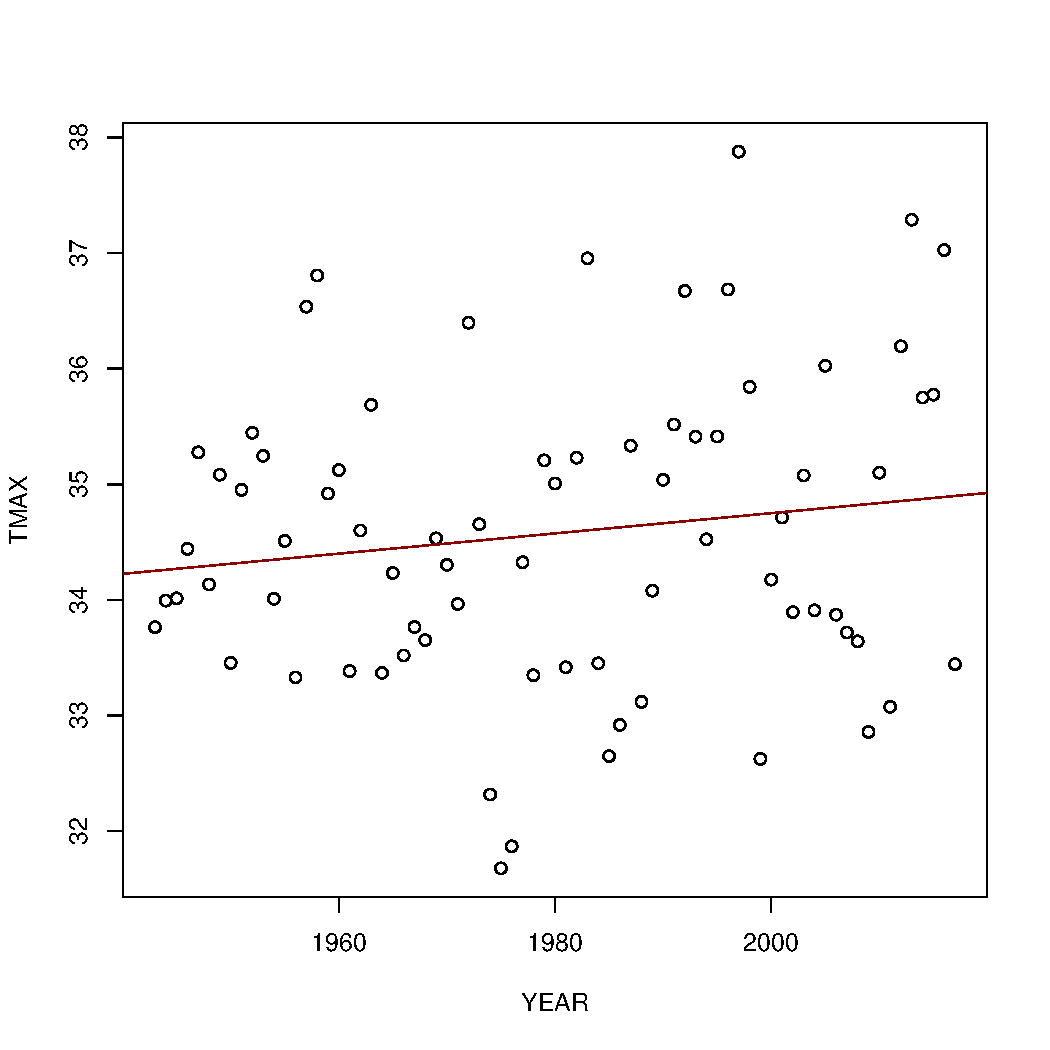
\includegraphics[width=\maxwidth]{figure/unnamed-chunk-7-1} 

\end{knitrout}

Let's fix the y-axis label as we did above (TMAX is not a very helpful label!). Furthermore, the x-axis needs to be calmed down some, so let's change the case for these. We will also change the symbols to make it less busy with the `pch' argument. You can look online to see the choices one has in R. 

I am also not impress with the vertical orientation of the y-axis, so it's important to change these as well. 

Finally, it's important that the image works in black and white. So, let's see if we can modify the graphic to make it less resource intensive. Finally, let's add a caption and reference to the figure (Figure \ref{fig:maxtemp}).

\begin{figure}[h]
\begin{knitrout}
\definecolor{shadecolor}{rgb}{0.969, 0.969, 0.969}\color{fgcolor}\begin{kframe}
\begin{alltt}
\hlstd{ylabel} \hlkwb{<-} \hlstr{"Maximum Temperature (°C)"}
\hlkwd{plot}\hlstd{(TMAX} \hlopt{~} \hlstd{YEAR,} \hlkwc{data}\hlstd{=MonthlyTMAXMean[MonthlyTMAXMean}\hlopt{$}\hlstd{MONTH}\hlopt{==}\hlnum{5}\hlstd{,],}
     \hlkwc{ylab}\hlstd{=ylabel,} \hlkwc{xlab}\hlstd{=}\hlstr{'Year'}\hlstd{,} \hlkwc{pch}\hlstd{=}\hlnum{20}\hlstd{,} \hlkwc{las}\hlstd{=}\hlnum{1}\hlstd{,} \hlkwc{col}\hlstd{=}\hlstr{'gray'}\hlstd{)}

\hlkwd{abline}\hlstd{(}\hlkwd{coef}\hlstd{(}\hlkwd{lm}\hlstd{(TMAX} \hlopt{~} \hlstd{YEAR,}
    \hlkwc{data}\hlstd{=MonthlyTMAXMean[MonthlyTMAXMean}\hlopt{$}\hlstd{MONTH}\hlopt{==}\hlnum{5}\hlstd{,])),} \hlkwc{col}\hlstd{=}\hlstr{'black'}\hlstd{)}
\end{alltt}
\end{kframe}
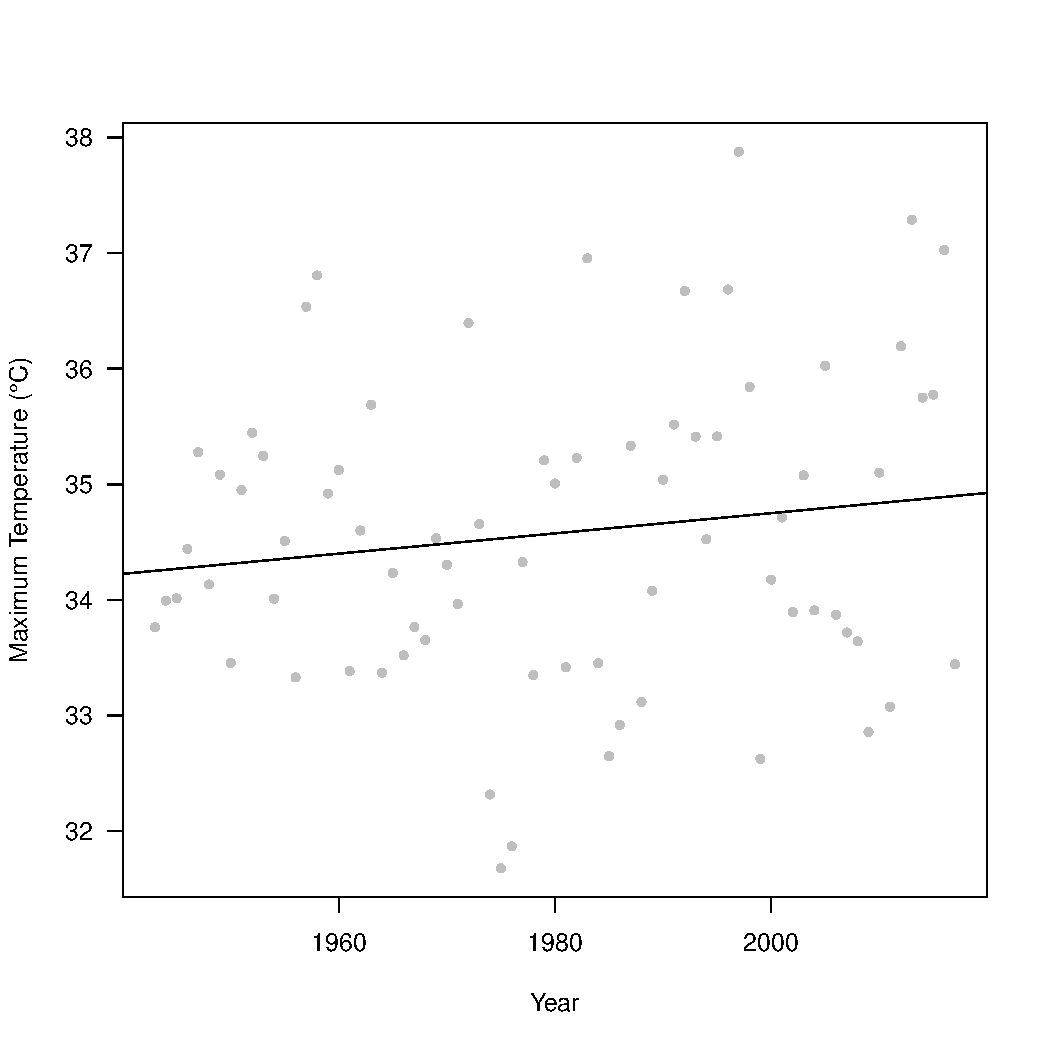
\includegraphics[width=\maxwidth]{figure/unnamed-chunk-8-1} 

\end{knitrout}
\caption{Monthly Average of Daily Maximum Temperatures (\degree C).  Notice the slightly darker line in the x-axis for the middle section. I am not sure how to get rid of this, but it bugs me!}
\label{fig:maxtemp}
\end{figure}

\clearpage
Now, what if we only want to display part of the data. We can limit the x-axis range using the 'xlim' argument, where we create a vector of for the start and end of the range.  

%\begin{figure}[h]
\begin{knitrout}
\definecolor{shadecolor}{rgb}{0.969, 0.969, 0.969}\color{fgcolor}\begin{kframe}
\begin{alltt}
\hlstd{ylabel} \hlkwb{<-} \hlstr{"Maximum Temperature (°C)"}
\hlkwd{plot}\hlstd{(TMAX} \hlopt{~} \hlstd{YEAR,} \hlkwc{data}\hlstd{=MonthlyTMAXMean[MonthlyTMAXMean}\hlopt{$}\hlstd{MONTH}\hlopt{==}\hlnum{5}\hlstd{,],}
     \hlkwc{xlim}\hlstd{=}\hlkwd{c}\hlstd{(}\hlnum{1940}\hlstd{,} \hlnum{2000}\hlstd{),}
     \hlkwc{ylab}\hlstd{=ylabel,} \hlkwc{xlab}\hlstd{=}\hlstr{'Year'}\hlstd{,} \hlkwc{pch}\hlstd{=}\hlnum{20}\hlstd{,} \hlkwc{las}\hlstd{=}\hlnum{1}\hlstd{,} \hlkwc{col}\hlstd{=}\hlstr{'gray'}\hlstd{)}

\hlkwd{abline}\hlstd{(}\hlkwd{coef}\hlstd{(}\hlkwd{lm}\hlstd{(TMAX} \hlopt{~} \hlstd{YEAR,}
    \hlkwc{data}\hlstd{=MonthlyTMAXMean[MonthlyTMAXMean}\hlopt{$}\hlstd{MONTH}\hlopt{==}\hlnum{5}\hlstd{,])),} \hlkwc{col}\hlstd{=}\hlstr{'black'}\hlstd{)}
\end{alltt}
\end{kframe}\begin{figure}
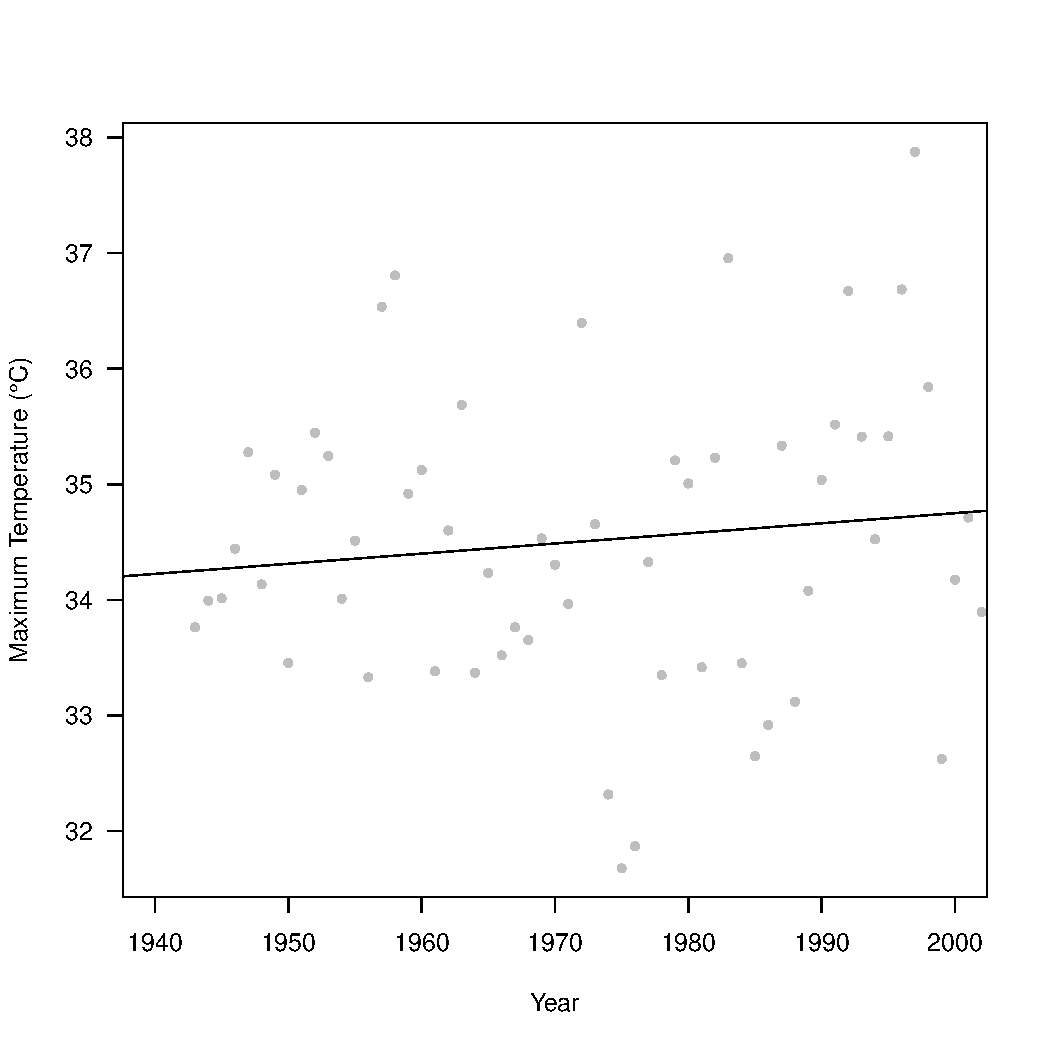
\includegraphics[width=\maxwidth]{figure/unnamed-chunk-9-1} \caption[Monthly Average of Daily Maximum Temperatures (C)]{Monthly Average of Daily Maximum Temperatures (C).}\label{fig:unnamed-chunk-9}
\end{figure}


\end{knitrout}
%\caption{Monthly Average of Daily Maximum Temperatures (\degree C).}
%\label{fig:maxtemp}
%\end{figure}

Alternatively, you may want to creat a best fit line that only covers the range for the existing data without extrapolating, which is usually a very good idea for most scientific endeavors!

For example, we have seen several papers that select parts of the record to make dubious claims. 

%\begin{figure}[ht]
\begin{knitrout}
\definecolor{shadecolor}{rgb}{0.969, 0.969, 0.969}\color{fgcolor}\begin{kframe}
\begin{alltt}
\hlstd{ylabel} \hlkwb{<-} \hlstr{"Maximum Temperature (°C)"}
\hlkwd{plot}\hlstd{(TMAX} \hlopt{~} \hlstd{YEAR,} \hlkwc{data}\hlstd{=MonthlyTMAXMean[MonthlyTMAXMean}\hlopt{$}\hlstd{MONTH}\hlopt{==}\hlnum{5}\hlstd{,],}
     \hlcom{#xlim=c(1940, 2000),}
     \hlkwc{ylab}\hlstd{=ylabel,} \hlkwc{xlab}\hlstd{=}\hlstr{'Year'}\hlstd{,} \hlkwc{pch}\hlstd{=}\hlnum{20}\hlstd{,} \hlkwc{las}\hlstd{=}\hlnum{1}\hlstd{,} \hlkwc{col}\hlstd{=}\hlstr{'gray'}\hlstd{)}

\hlstd{MonthlyTMAX.lm} \hlkwb{=} \hlstd{(}\hlkwd{lm}\hlstd{(TMAX} \hlopt{~} \hlstd{YEAR,}
    \hlkwc{data}\hlstd{=MonthlyTMAXMean[MonthlyTMAXMean}\hlopt{$}\hlstd{MONTH}\hlopt{==}\hlnum{5}\hlstd{, ]))}
\hlstd{interpolated} \hlkwb{=} \hlkwd{predict}\hlstd{(MonthlyTMAX.lm,}
      \hlstd{MonthlyTMAXMean[MonthlyTMAXMean}\hlopt{$}\hlstd{MONTH}\hlopt{==}\hlnum{5}\hlstd{,])}

\hlkwd{lines}\hlstd{(MonthlyTMAXMean}\hlopt{$}\hlstd{YEAR[MonthlyTMAXMean}\hlopt{$}\hlstd{MONTH}\hlopt{==}\hlnum{5}\hlstd{],}
      \hlstd{interpolated,} \hlkwc{col}\hlstd{=}\hlstr{'blue'}\hlstd{)}

\hlstd{MonthlyTMAX.lm2} \hlkwb{=} \hlstd{(}\hlkwd{lm}\hlstd{(TMAX} \hlopt{~} \hlstd{YEAR,}
    \hlkwc{data}\hlstd{=MonthlyTMAXMean[MonthlyTMAXMean}\hlopt{$}\hlstd{MONTH}\hlopt{==}\hlnum{5} \hlopt{&}
            \hlstd{MonthlyTMAXMean}\hlopt{$}\hlstd{YEAR}\hlopt{>}\hlnum{2000}\hlstd{, ]))}

\hlstd{interpolated2} \hlkwb{=} \hlkwd{predict}\hlstd{(MonthlyTMAX.lm2,}
            \hlstd{MonthlyTMAXMean[MonthlyTMAXMean}\hlopt{$}\hlstd{MONTH}\hlopt{==}\hlnum{5} \hlopt{&}
            \hlstd{MonthlyTMAXMean}\hlopt{$}\hlstd{YEAR}\hlopt{>}\hlnum{2000}\hlstd{,])}

\hlkwd{lines}\hlstd{(MonthlyTMAXMean}\hlopt{$}\hlstd{YEAR[MonthlyTMAXMean}\hlopt{$}\hlstd{MONTH}\hlopt{==}\hlnum{5} \hlopt{&}
            \hlstd{MonthlyTMAXMean}\hlopt{$}\hlstd{YEAR}\hlopt{>}\hlnum{2000}\hlstd{], interpolated2,} \hlkwc{col}\hlstd{=}\hlstr{'red'}\hlstd{)}

\hlkwd{legend}\hlstd{(}\hlnum{1948}\hlstd{,} \hlnum{38}\hlstd{,} \hlkwc{legend}\hlstd{=}\hlkwd{c}\hlstd{(}\hlstr{"1952-2018 Record"}\hlstd{,} \hlstr{"2000-2018 Record"}\hlstd{),}
       \hlkwc{lty}\hlstd{=}\hlnum{1}\hlstd{,} \hlkwc{col}\hlstd{=}\hlkwd{c}\hlstd{(}\hlstr{"blue"}\hlstd{,} \hlstr{"red"}\hlstd{))}
\end{alltt}
\end{kframe}
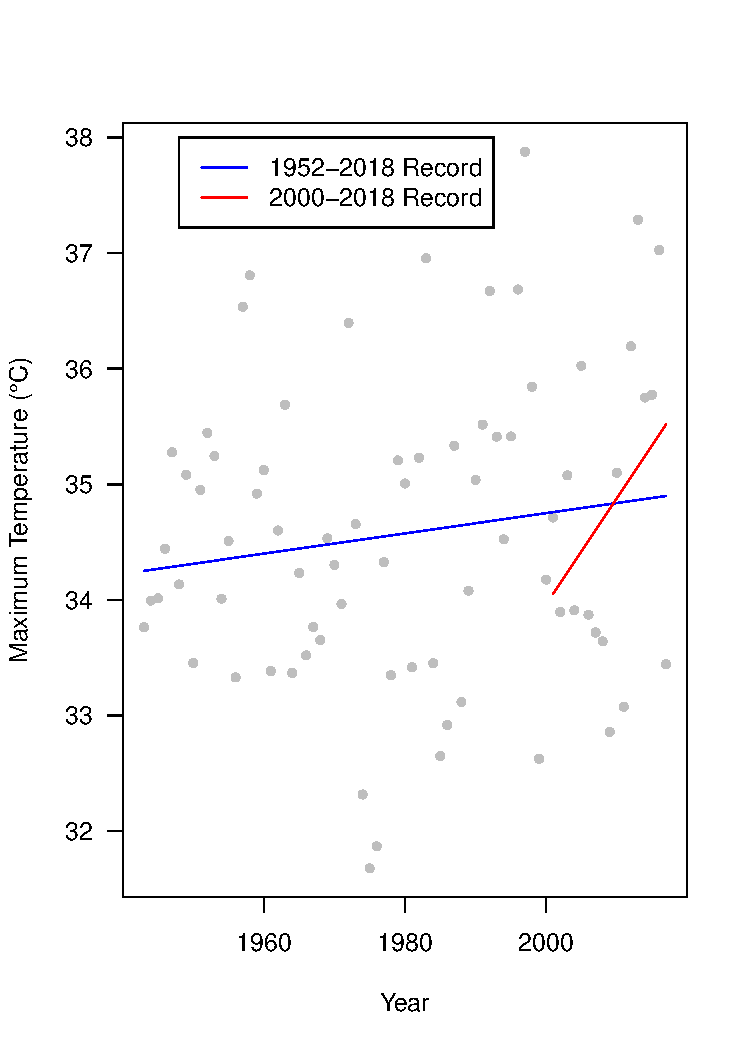
\includegraphics[width=\maxwidth]{figure/fig_height__3-1} 

\end{knitrout}
%\caption{Monthly Average of Daily Maximum Temperatures (\degree C).}
%\label{fig:maxtemp}
%\end{figure}


\clearpage
\section{Bar Graphs}

Rainfall data and other types of 'count' data are often best displayed as barcharts. 


\begin{knitrout}
\definecolor{shadecolor}{rgb}{0.969, 0.969, 0.969}\color{fgcolor}\begin{kframe}
\begin{alltt}
\hlstd{fires} \hlkwb{=} \hlkwd{data.frame}\hlstd{(}\hlkwc{Year} \hlstd{=} \hlnum{2010}\hlopt{:}\hlnum{2018}\hlstd{,}
                   \hlkwc{Fires} \hlstd{=} \hlkwd{c}\hlstd{(}\hlnum{1}\hlstd{,} \hlnum{0}\hlstd{,} \hlnum{2}\hlstd{,} \hlnum{0}\hlstd{,} \hlnum{1}\hlstd{,} \hlnum{13}\hlstd{,} \hlnum{0}\hlstd{,} \hlnum{16}\hlstd{,} \hlnum{13}\hlstd{))}
\hlcom{# Note: barplot uses names.arg to assign the category names}
\hlkwd{barplot}\hlstd{(fires}\hlopt{$}\hlstd{Fires,} \hlkwc{names.arg} \hlstd{= fires}\hlopt{$}\hlstd{Year,} \hlkwc{las}\hlstd{=}\hlnum{1}\hlstd{,} \hlkwc{ylab}\hlstd{=}\hlstr{"No. of Fires"}\hlstd{)}
\end{alltt}
\end{kframe}\begin{figure}
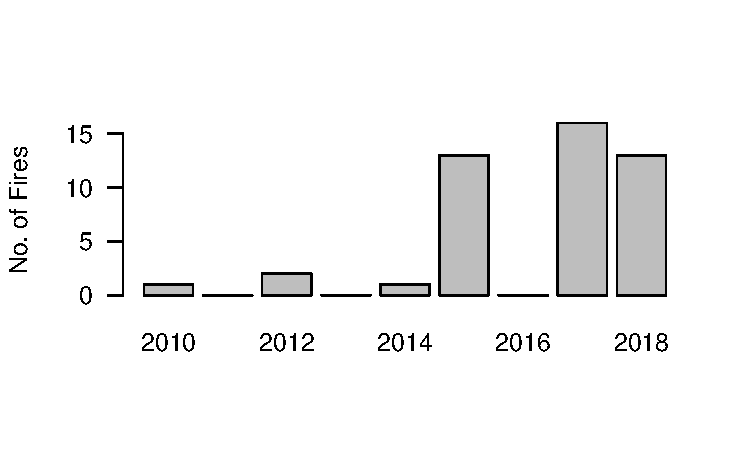
\includegraphics[width=\maxwidth]{figure/unnamed-chunk-10-1} \caption[Number of Unsafe Air Quality Days in Washington State due to Fires]{Number of Unsafe Air Quality Days in Washington State due to Fires.}\label{fig:unnamed-chunk-10}
\end{figure}


\end{knitrout}


Notice the figure cuts out every-other year. You'll need to decide if the reader will be bothered by that. If so, you can reduce the x-axis labels fonts or increase the width of the chart. 

\section{Tables}

Sometimes (often times?), tables are better than graphs. In the case below, I summarized the grades for each set of drafts using a table and a histogram. 




\begin{kframe}
\begin{alltt}
\hlkwd{print}\hlstd{(}\hlkwd{xtable}\hlstd{(grades.df,}
      \hlkwc{caption}\hlstd{=}\hlstr{'Table of First Blog Draft Scores'}\hlstd{),}
      \hlkwc{caption.placement} \hlstd{=} \hlstr{"top"}\hlstd{)}
\end{alltt}
\end{kframe}% latex table generated in R 3.4.1 by xtable 1.8-2 package
% 
\begin{tabular}{rlrr}
  \hline
 & Range & 1st Draft & 2nd Draft \\ 
  \hline
1 & (0,10] &   3 &   0 \\ 
  2 & (10,20] &   0 &   3 \\ 
  3 & (20,30] &   7 &   0 \\ 
  4 & (30,40] &   4 &   4 \\ 
  5 & (40,50] &   0 &   0 \\ 
   \hline
\end{tabular}


The histogram is simple, but for these data, I am not sure it's all that useful. Which do you think is more effective?

\bigskip
BTW: The mean was for the first draft was 21.1 and the second draft was 27.6. You will have 5 opportunities to re-submit to improve your grade, but only two weeks to accomplish this. Since it takes two days to read them, you'll need to submit every 2 days if you want to take full advange of this opportunity. 

\bigskip
\begin{knitrout}
\definecolor{shadecolor}{rgb}{0.969, 0.969, 0.969}\color{fgcolor}\begin{kframe}
\begin{alltt}
\hlkwd{par}\hlstd{(}\hlkwc{mfrow}\hlstd{=}\hlkwd{c}\hlstd{(}\hlnum{1}\hlstd{,}\hlnum{2}\hlstd{))}
\hlkwd{hist}\hlstd{(grades1,} \hlkwc{main}\hlstd{=}\hlstr{"1st Draft"}\hlstd{,} \hlkwc{xlab}\hlstd{=}\hlstr{"Score"}\hlstd{,}
     \hlkwc{xlim}\hlstd{=}\hlkwd{c}\hlstd{(}\hlnum{0}\hlstd{,}\hlnum{50}\hlstd{),} \hlkwc{col}\hlstd{=}\hlstr{"green"}\hlstd{)}
\hlkwd{hist}\hlstd{(grades2,} \hlkwc{main}\hlstd{=}\hlstr{"2nd Draft"}\hlstd{,} \hlkwc{xlab}\hlstd{=}\hlstr{"Score"}\hlstd{,}
     \hlkwc{xlim}\hlstd{=}\hlkwd{c}\hlstd{(}\hlnum{0}\hlstd{,}\hlnum{50}\hlstd{),} \hlkwc{col}\hlstd{=}\hlstr{"blue"}\hlstd{)}
\end{alltt}
\end{kframe}\begin{figure}
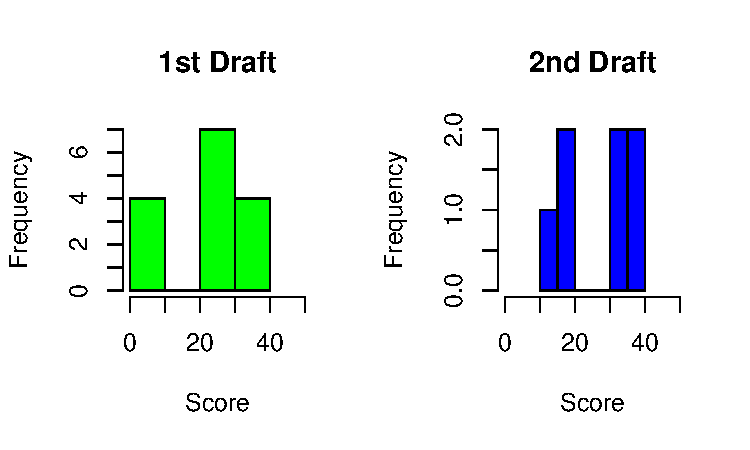
\includegraphics[width=\maxwidth]{figure/unnamed-chunk-13-1} \caption[Histogram of Blog Scores]{Histogram of Blog Scores}\label{fig:unnamed-chunk-13}
\end{figure}


\end{knitrout}

\begin{knitrout}
\definecolor{shadecolor}{rgb}{0.969, 0.969, 0.969}\color{fgcolor}\begin{kframe}
\begin{alltt}
\hlcom{# Display the Student's t distributions with various}
\hlcom{# degrees of freedom and compare to the normal distribution}
\hlstd{x} \hlkwb{=} \hlkwd{seq}\hlstd{(}\hlnum{0}\hlstd{,} \hlnum{50}\hlstd{,} \hlkwc{by} \hlstd{=} \hlnum{2}\hlstd{)}
\hlstd{hx1} \hlkwb{<-} \hlkwd{dnorm}\hlstd{(}\hlkwc{x}\hlstd{= x,} \hlkwc{mean} \hlstd{=} \hlkwd{mean}\hlstd{(grades1,} \hlkwc{na.rm}\hlstd{=T),}
             \hlkwc{sd}\hlstd{=}\hlkwd{sd}\hlstd{(grades1,} \hlkwc{na.rm}\hlstd{=T))}
\hlstd{hx2} \hlkwb{<-} \hlkwd{dnorm}\hlstd{(}\hlkwc{x}\hlstd{= x,} \hlkwc{mean} \hlstd{=} \hlkwd{mean}\hlstd{(grades2,} \hlkwc{na.rm}\hlstd{=T),}
             \hlkwc{sd}\hlstd{=} \hlkwd{sd}\hlstd{(grades2,} \hlkwc{na.rm}\hlstd{=T))}

\hlstd{colors} \hlkwb{<-} \hlkwd{c}\hlstd{(}\hlstr{"red"}\hlstd{,} \hlstr{"blue"}\hlstd{,} \hlstr{"darkgreen"}\hlstd{,} \hlstr{"gold"}\hlstd{,} \hlstr{"black"}\hlstd{)}
\hlstd{labels} \hlkwb{<-} \hlkwd{c}\hlstd{(}\hlstr{"Draft 1"}\hlstd{,} \hlstr{"Draft 2"}\hlstd{,} \hlstr{"Draft 3"}\hlstd{,} \hlstr{"Draft 4"}\hlstd{,} \hlstr{"Draft 5"}\hlstd{)}

\hlkwd{plot}\hlstd{(x, hx1,} \hlkwc{type}\hlstd{=}\hlstr{"l"}\hlstd{,} \hlkwc{lty}\hlstd{=}\hlnum{1}\hlstd{,} \hlkwc{xlab}\hlstd{=}\hlstr{"Score"}\hlstd{,}
  \hlkwc{ylab}\hlstd{=}\hlstr{"Density"}\hlstd{,} \hlkwc{main}\hlstd{=}\hlstr{"Distribution of Scores"}\hlstd{,} \hlkwc{las}\hlstd{=}\hlnum{1}\hlstd{,}
  \hlkwc{ylim}\hlstd{=}\hlkwd{c}\hlstd{(}\hlnum{0}\hlstd{,}\hlnum{.1}\hlstd{),} \hlkwc{col}\hlstd{=colors[}\hlnum{1}\hlstd{])}
  \hlkwd{lines}\hlstd{(x, hx2,} \hlkwc{lwd}\hlstd{=}\hlnum{2}\hlstd{,} \hlkwc{col}\hlstd{=colors[}\hlnum{2}\hlstd{])}

\hlstd{ttest} \hlkwb{=} \hlkwd{t.test}\hlstd{(grades1, grades2)}

\hlkwd{text}\hlstd{(ttest}\hlopt{$}\hlstd{estimate[}\hlnum{1}\hlstd{],} \hlkwd{max}\hlstd{(hx1),} \hlstr{"Draft 1 Mean"}\hlstd{,} \hlkwc{pos}\hlstd{=}\hlnum{3}\hlstd{)}
\hlkwd{text}\hlstd{(ttest}\hlopt{$}\hlstd{estimate[}\hlnum{2}\hlstd{],} \hlkwd{max}\hlstd{(hx2),} \hlstr{"Draft 2 Mean"}\hlstd{,} \hlkwc{pos}\hlstd{=}\hlnum{3}\hlstd{)}

\hlkwd{text}\hlstd{(}\hlnum{10}\hlstd{,} \hlnum{.07}\hlstd{,} \hlkwd{paste}\hlstd{(}\hlstr{"p-value = "}\hlstd{,} \hlkwd{round}\hlstd{(ttest}\hlopt{$}\hlstd{p.value,} \hlnum{3}\hlstd{)))}
\hlkwd{legend}\hlstd{(}\hlstr{"topright"}\hlstd{,} \hlkwc{inset}\hlstd{=}\hlnum{.05}\hlstd{,} \hlkwc{title}\hlstd{=}\hlstr{"Distributions"}\hlstd{,}
  \hlstd{labels,} \hlkwc{lwd}\hlstd{=}\hlnum{2}\hlstd{,} \hlkwc{lty}\hlstd{=}\hlkwd{c}\hlstd{(}\hlnum{1}\hlstd{,} \hlnum{1}\hlstd{,} \hlnum{1}\hlstd{,} \hlnum{1}\hlstd{,} \hlnum{1}\hlstd{),} \hlkwc{col}\hlstd{=colors)}
\end{alltt}
\end{kframe}\begin{figure}
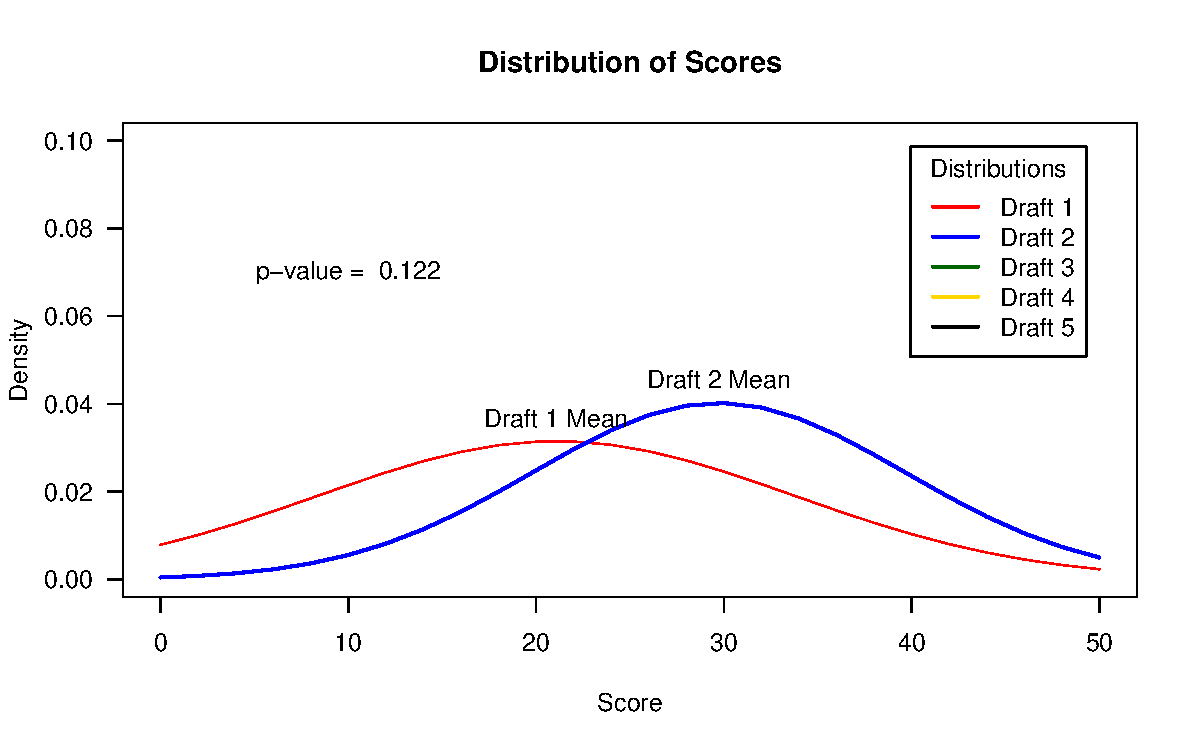
\includegraphics[width=\maxwidth]{figure/unnamed-chunk-14-1} \caption[Probability Density for Scores]{Probability Density for Scores}\label{fig:unnamed-chunk-14}
\end{figure}


\end{knitrout}

\end{document}
